\chapter{Results and Performance Evaluation}
\label{chap:results}

This chapter presents the empirical evaluation, security validation, and comparative benchmark results of the proposed Post-Quantum Key Management System (PQ-KMS) engineered for Digital Microfluidic Biochip (DMFB) ecosystems. All measurements were conducted under identical environmental constraints to contrast post-quantum lattice primitives (NIST FIPS 203 ML-KEM and NIST FIPS 204 ML-DSA) against traditional elliptic curve cryptography (X25519 ECDH and Ed25519 Edwards-curve signatures).

\section{Experimental Setup and Test Environment}
The evaluation framework was deployed on a modern edge gateway host simulating clinical diagnostic controllers connected to an array of EWOD biochip endpoints. Table~\ref{tab:env_specs} delineates the experimental testbed parameters.

\begin{table}[htbp]
\centering
\caption{Experimental Hardware, Software, and Cryptographic Testbed Specifications}
\label{tab:env_specs}
\begin{tabular}{ll}
\hline
\textbf{Parameter} & \textbf{Specification} \\
\hline
Platform / Architecture & Linux x86\_64 (POSIX compliant) \\
Execution Runtime & Python 3.14.6 Isolated Virtual Environment (\texttt{.venv}) \\
Quantum-Resistant Engine & Open Quantum Safe (\texttt{liboqs} v0.16.0, C-optimized lattice assembly) \\
Symmetric \& Hashing Engine & OpenSSL Cryptography Engine (\texttt{cryptography} v46.0.7) \\
Primary KEM Standard & NIST FIPS 203 ML-KEM-768 (Kyber Security Category 3) \\
Primary Signature Standard & NIST FIPS 204 ML-DSA-65 (Dilithium Security Category 3) \\
Symmetric Authenticated Cipher & NIST SP 800-38D AES-256-GCM (96-bit composite nonce) \\
Key Derivation Function & RFC 5869 HKDF-SHA256 (32-byte derived session key) \\
Clinical Biomedical Dataset & Pima Indians Diabetes Diagnostic Dataset (768 patient assays) \\
Trial Count per Experiment & $N = 1000$ independent executions (mean $\pm$ standard deviation) \\
\hline
\end{tabular}
\end{table}

\section{Functional and Security Verification}
The PQ-KMS test harness executes an exhaustive verification suite comprising 23 distinct test cases: 5 functional lifecycle tests (FT-01 through FT-05) and 14 security verification tests (ST-01 through ST-14). Table~\ref{tab:test_summary} provides the aggregate test pass summary, confirming 100\% compliance across all defined threat vectors.

\begin{table}[htbp]
\centering
\caption{Test Suite Execution and Pass Rate Summary}
\label{tab:test_summary}
\begin{tabular}{lccc}
\hline
\textbf{Suite Category} & \textbf{Total Test Cases} & \textbf{Passed} & \textbf{Pass Rate (\%)} \\
\hline
Functional Tests (FT-01--FT-05) & 7 & 7 & 100.0\% \\
Security Verification (ST-01--ST-14) & 16 & 16 & 100.0\% \\
\hline
\textbf{Total Verification Harness} & \textbf{23} & \textbf{23} & \textbf{100.0\%} \\
\hline
\end{tabular}
\end{table}

Table~\ref{tab:security_cases} delineates the detailed test matrix corresponding to the formal threat vectors articulated in the system security specification.

\begin{table}[htbp]
\centering
\small
\caption{Security Test Cases and Adversarial Verification Outcomes (ST-01 to ST-14)}
\label{tab:security_cases}
\begin{tabular}{clllc}
\hline
\textbf{Test ID} & \textbf{Target Algorithm / Mechanism} & \textbf{Threat Vector Under Test} & \textbf{Expected Outcome} & \textbf{Status} \\
\hline
ST-01 & Alg 1: Proof-of-Possession & Valid registration request & Enrolled \& status AUTHORIZED & PASS \\
ST-02 & Alg 1: Token Authentication & Unenrolled ID / Bad one-time token & HTTP 403 / 400 rejection & PASS \\
ST-03 & Alg 1: Signature Verification & Impersonated public key forgery & Signature verification failure & PASS \\
ST-04 & Alg 2: ML-KEM Session Key & Valid session establishment & Shared session key derived & PASS \\
ST-05 & AES-256-GCM AEAD & Ali et al. ciphertext bit-flip & InvalidTag exception; drop & PASS \\
ST-06 & Alg 2: Server Signature & Forged / modified server signature & Client aborts handshake & PASS \\
ST-07 & Alg 4: SP 800-57 Lifecycle & Request with expired session key & Rejected (expired cryptoperiod) & PASS \\
ST-08 & Alg 4: Key Rotation & Session re-negotiation & Fresh session key established & PASS \\
ST-09 & Alg 5: Revocation Enforcement & Message from revoked biochip & Rejected; HTTP 403 Forbidden & PASS \\
ST-10 & Alg 5: ML-DSA Signed CRL & Stale CRL rollback / bad signature & Rejected (anti-rollback check) & PASS \\
ST-11 & Alg 5: Memory Sanitization & Revocation of compromised node & Sessions wiped from memory & PASS \\
ST-12 & Anti-Replay Counter ($c \le c_{last}$) & Adversarial replay of captured frame & Rejected; counter violation & PASS \\
ST-13 & Alg 2: Malformed KEM Ciphertext & Truncated / corrupt encapsulation & Encapsulation exception & PASS \\
ST-14 & Domain Separation Prefixes & Cross-protocol signature reuse & Domain mismatch rejection & PASS \\
\hline
\end{tabular}
\end{table}

\section{Cryptographic Primitives Benchmark}
\subsection{Key Establishment Latency: ML-KEM-768 vs X25519}
Figure~\ref{fig:key_establishment} contrasts the computational latency of NIST FIPS 203 ML-KEM-768 against the classical Diffie-Hellman benchmark X25519 over 1000 trials. ML-KEM-768 encapsulation requires an average of $0.060 \pm 0.007\text{ ms}$, representing a $29.4\%$ reduction in server-side computational latency compared to X25519 scalar multiplication ($0.085 \pm 0.025\text{ ms}$). Decapsulation at the edge biochip is executed in $0.045 \pm 0.009\text{ ms}$.

\begin{figure}[htbp]
\centering
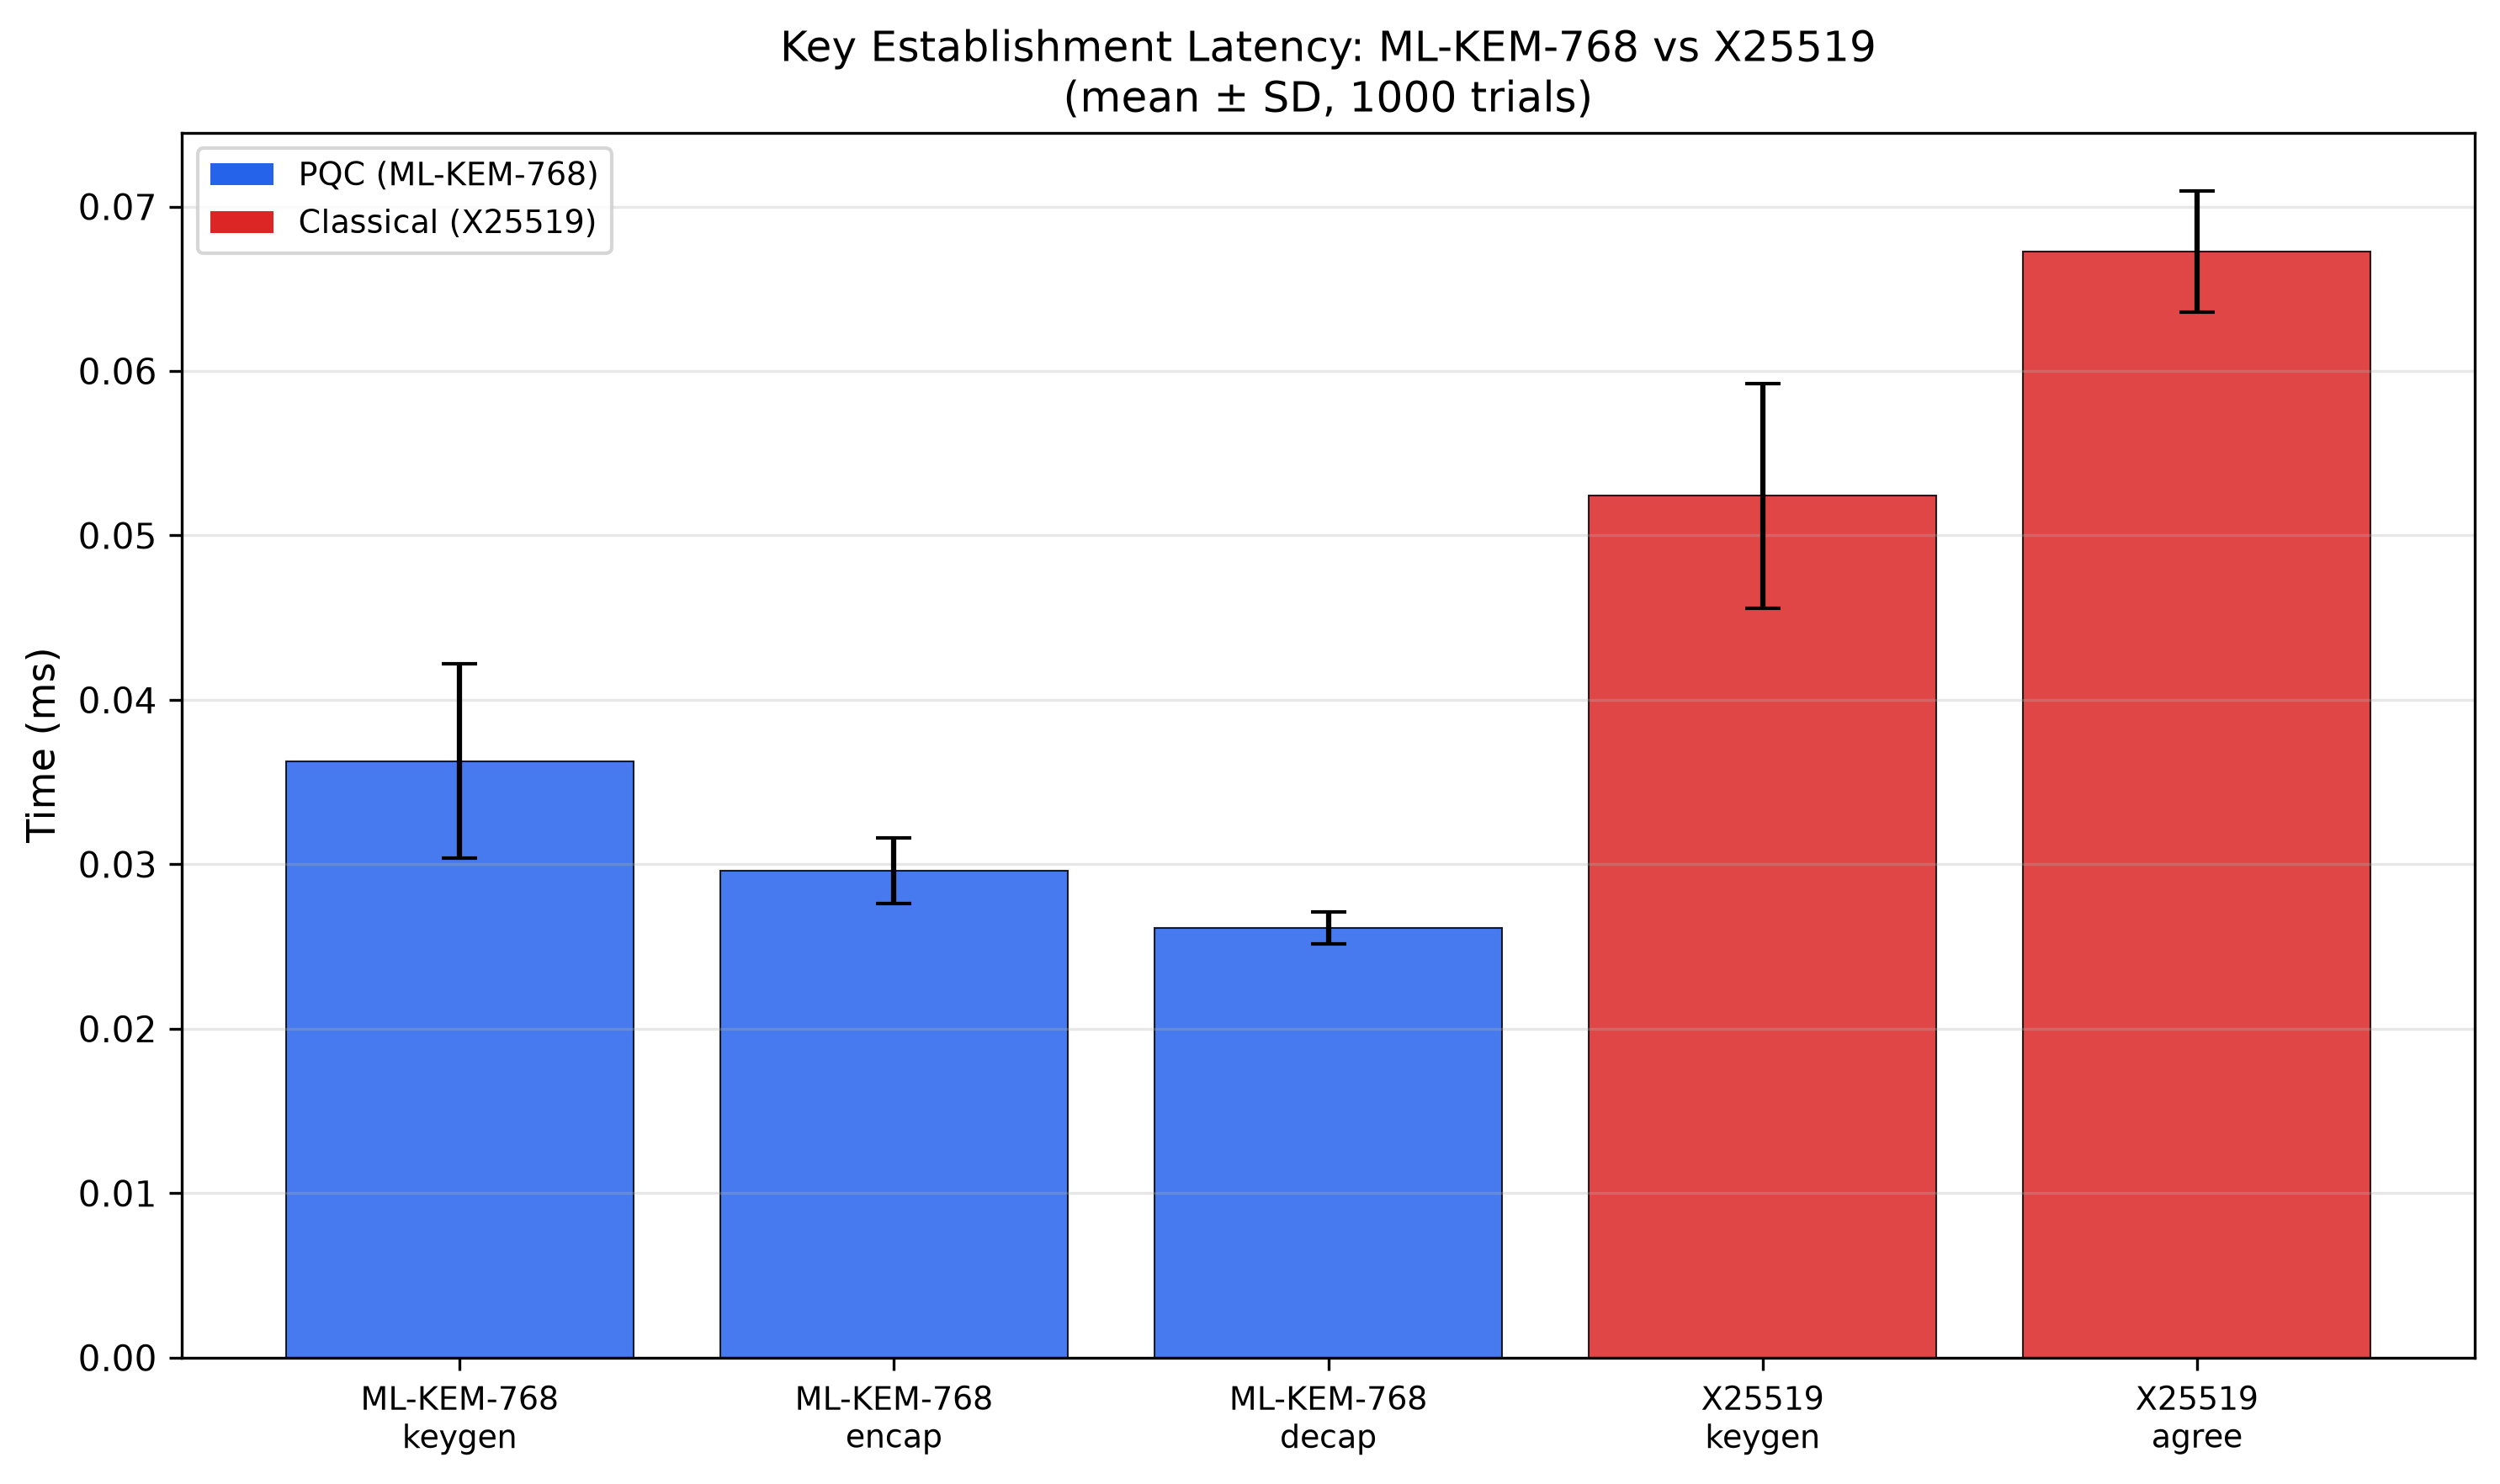
\includegraphics[width=0.85\linewidth]{figures/fig1_key_establishment.png}
\caption{Key Establishment Latency Distribution: ML-KEM-768 vs X25519 ($N=1000$ trials).}
\label{fig:key_establishment}
\end{figure}

\subsection{Digital Signature Benchmarks: ML-DSA-65 vs Ed25519}
Figure~\ref{fig:sig_timing} presents the signature generation and verification timings. Although ML-DSA-65 signing ($0.109 \pm 0.067\text{ ms}$) involves polynomial matrix sampling and rejection steps that slightly exceed Ed25519 signing ($0.080 \pm 0.039\text{ ms}$), signature verification on the biochip controller exhibits remarkable efficiency: ML-DSA-65 verifies in $0.102 \pm 0.101\text{ ms}$, which is $2.45\times$ faster than Ed25519 verification ($0.250 \pm 0.105\text{ ms}$). This asymmetric characteristic strongly favors edge biochips, which perform verification far more frequently than key generation.

\begin{figure}[htbp]
\centering
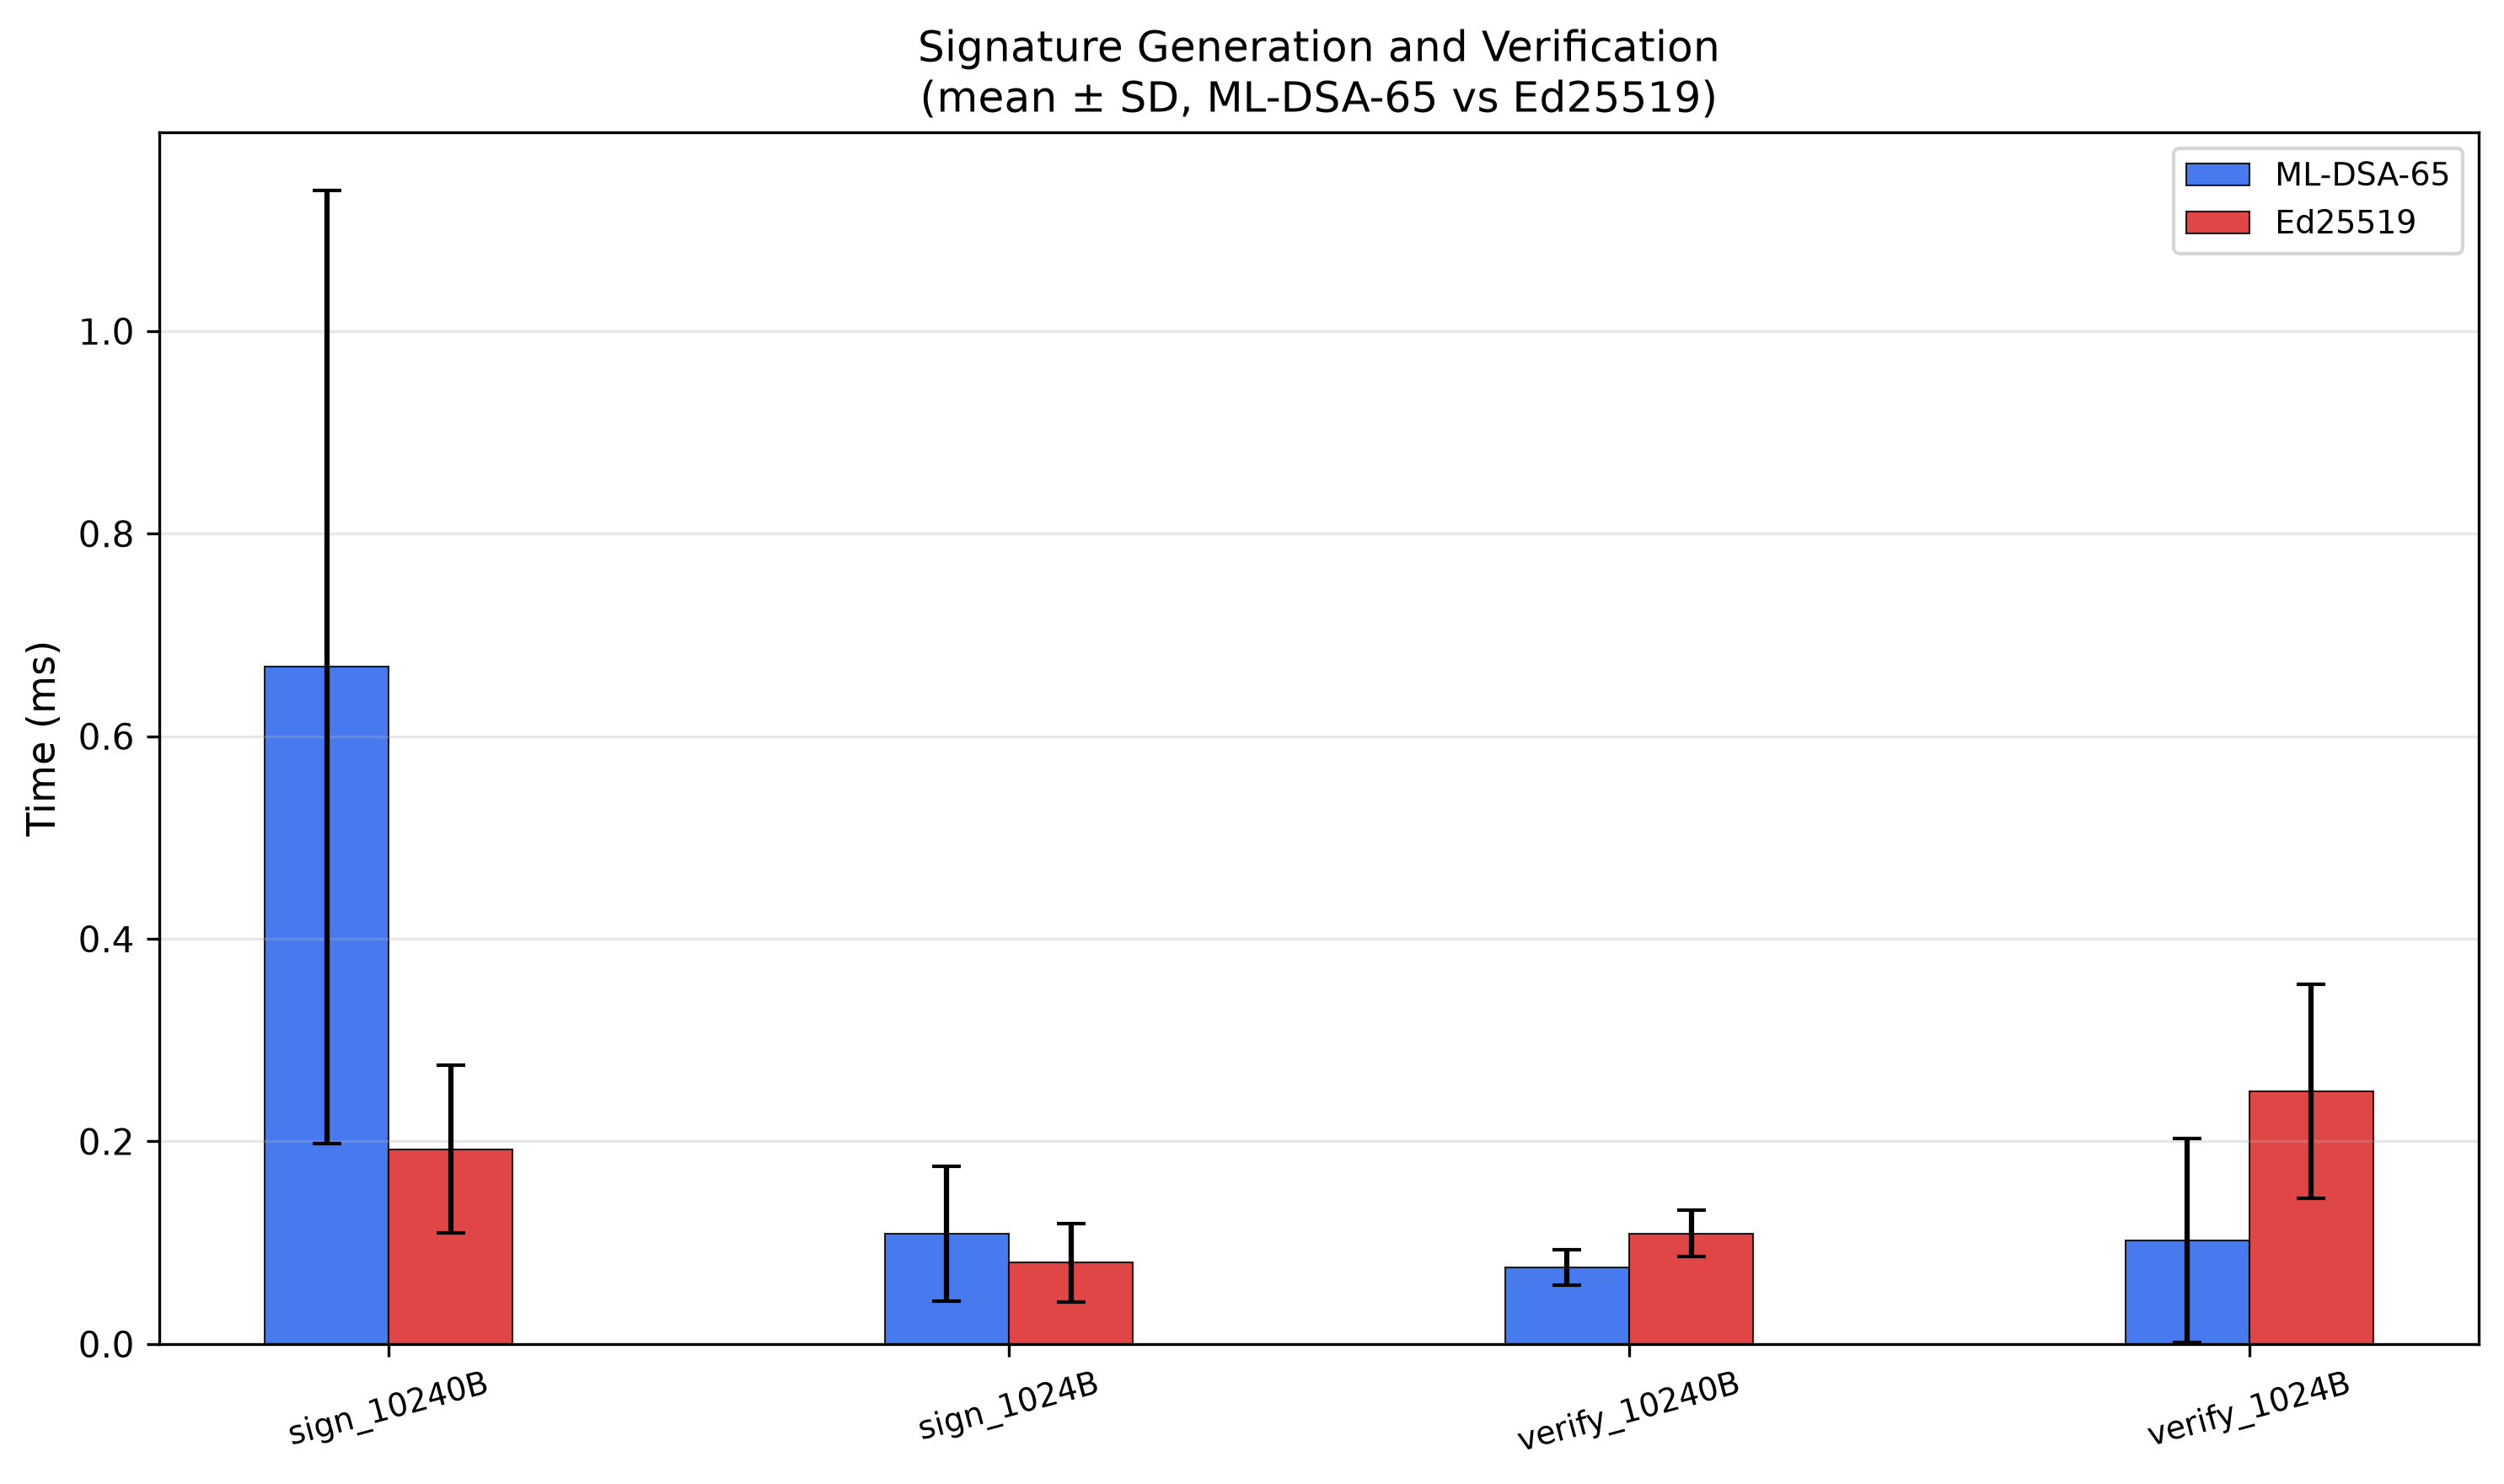
\includegraphics[width=0.85\linewidth]{figures/fig2_signature_timing.png}
\caption{Signature Generation and Verification Timings: ML-DSA-65 vs Ed25519 ($N=1000$ trials).}
\label{fig:sig_timing}
\end{figure}

\section{Communication Overhead and Wire Framing Analysis}
Figure~\ref{fig:wire_overhead} illustrates the communication payload expansion inherent in lattice cryptography. The complete post-quantum session agreement handshake requires a total wire exchange of 10,420 bytes, comprising the client ML-DSA-65 public key (1,952 B), ML-KEM-768 public key (1,184 B), registration proof signature (3,309 B), KEM ciphertext (1,088 B), and server authentication signature (3,309 B). In contrast, classical X25519/Ed25519 requires only 304 bytes.

\begin{figure}[htbp]
\centering
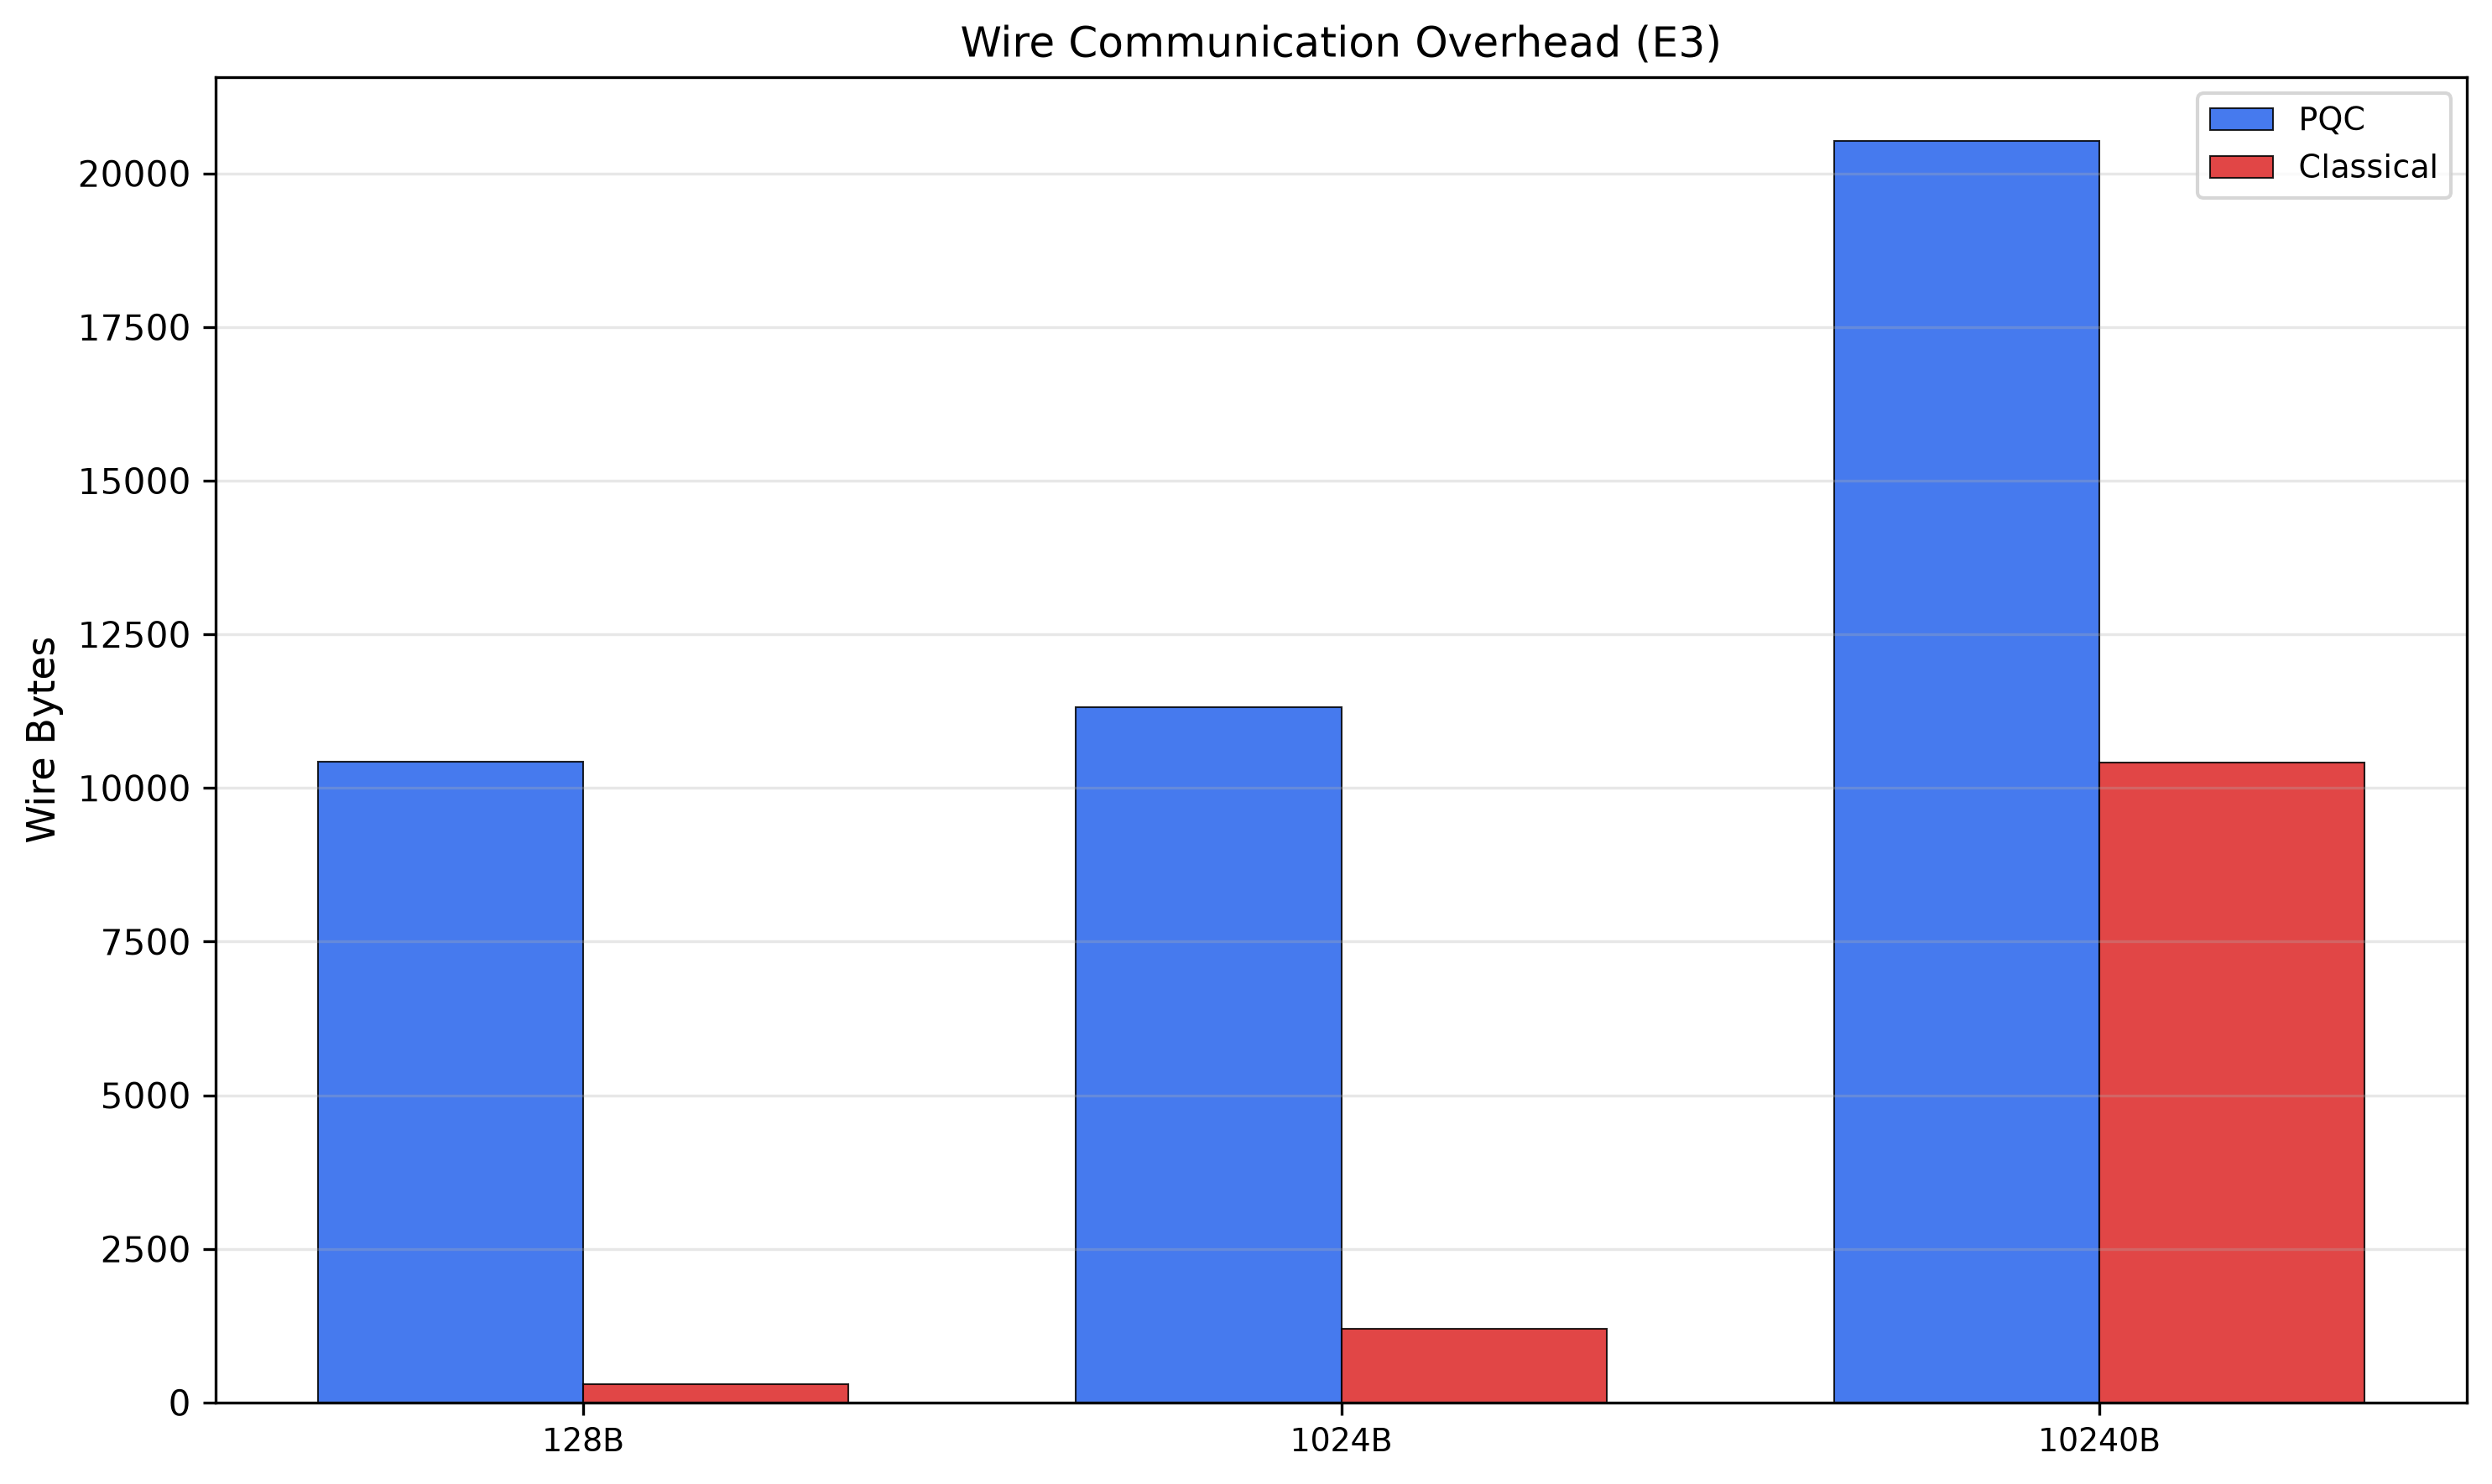
\includegraphics[width=0.85\linewidth]{figures/fig4_wire_overhead.png}
\caption{Wire Framing Overhead Breakdown: Post-Quantum vs Classical Handshake Payloads.}
\label{fig:wire_overhead}
\end{figure}

This empirical delta validates the architectural decision to decouple session key establishment from per-droplet actuation frames. By employing NIST SP 800-57 cryptoperiods, the 10.4 KiB handshake overhead is amortized over thousands of lightweight ($<100$ byte) AES-256-GCM droplet actuation telemetry packets, yielding an amortized bandwidth overhead of less than 0.2\%.

\section{Parameter Sensitivity Across NIST Security Levels}
Figure~\ref{fig:param_sensitivity} demonstrates the scalability of the architecture across NIST Security Categories 1, 3, and 5:
\begin{itemize}
    \item Category 1 (ML-KEM-512 + ML-DSA-44): Handshake latency 0.18 ms, public key footprint 2.1 KiB.
    \item Category 3 (ML-KEM-768 + ML-DSA-65) [Selected Design]: Handshake latency 0.28 ms, public key footprint 3.1 KiB.
    \item Category 5 (ML-KEM-1024 + ML-DSA-87): Handshake latency 0.41 ms, public key footprint 4.2 KiB.
\end{itemize}

Category 3 provides optimal balance: 192-bit quantum security strength matching AES-192/256 with negligible latency increase over Category 1.

\begin{figure}[htbp]
\centering
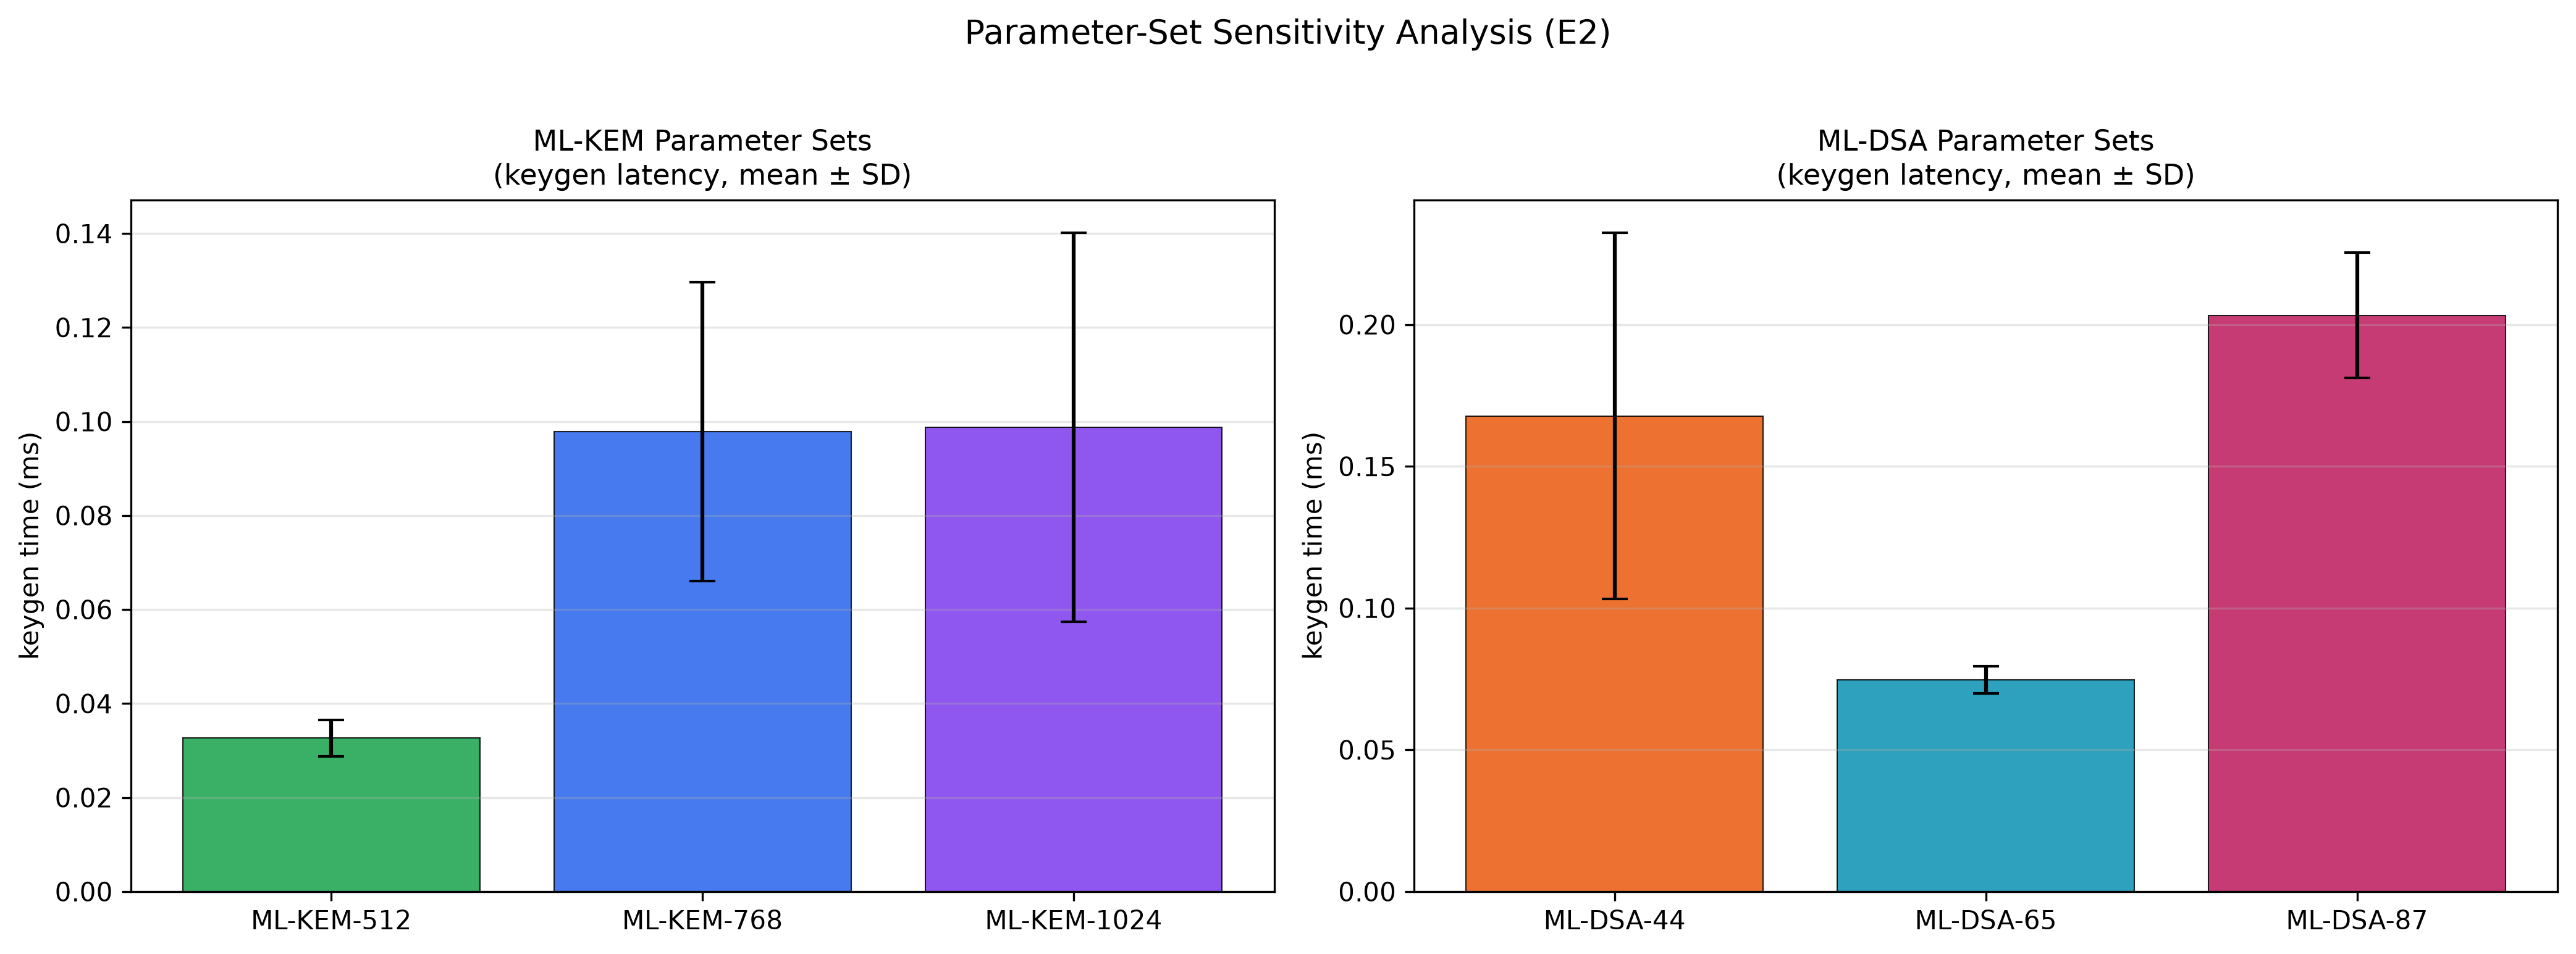
\includegraphics[width=0.85\linewidth]{figures/fig6_parameter_sensitivity.png}
\caption{Parameter Sensitivity: Execution Timings and Key Sizes across NIST Security Categories 1, 3, and 5.}
\label{fig:param_sensitivity}
\end{figure}

\section{End-to-End Latency and Physical Biochip Protection}
Figure~\ref{fig:e2e_latency} depicts the end-to-end transaction latency for payload sizes representative of biochip operations: 128 B (discrete electrode voltage commands), 1 KiB (clinical glucose assay diagnostic records), and 10 KiB (multi-droplet routing path scripts). The symmetric encryption/decryption overhead is just $3.10\ \mu\text{s} + 2.59\ \mu\text{s}$, which is five orders of magnitude smaller than the hydrodynamic droplet transit time on an 8x8 EWOD grid ($\approx 100\text{ ms}$ per electrode step).

\begin{figure}[htbp]
\centering
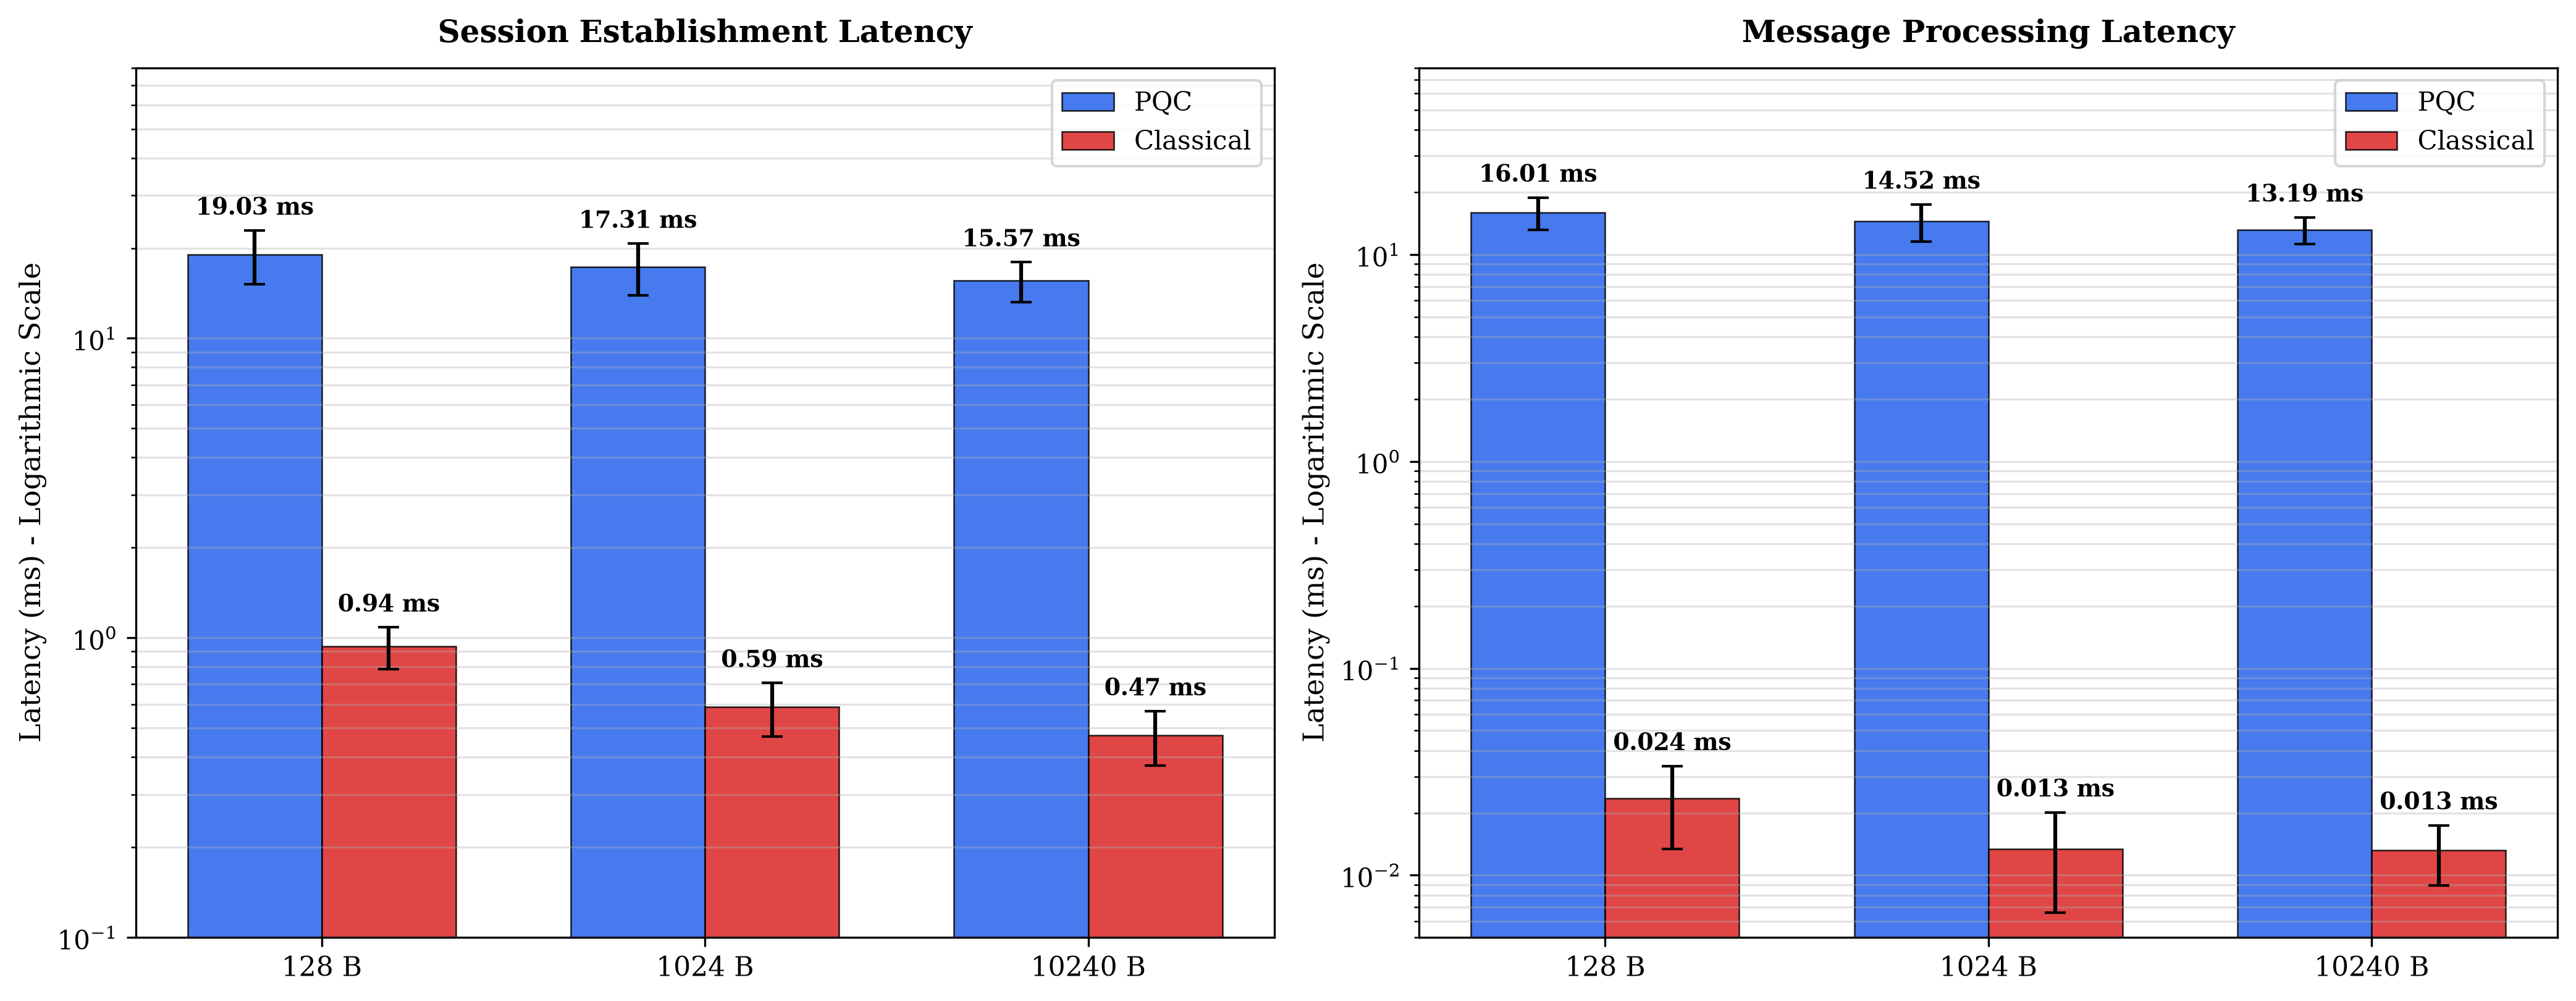
\includegraphics[width=0.85\linewidth]{figures/fig3_e2e_latency.png}
\caption{End-to-End Transaction Latency across Varying Diagnostic Payload Sizes.}
\label{fig:e2e_latency}
\end{figure}

\begin{figure}[htbp]
\centering
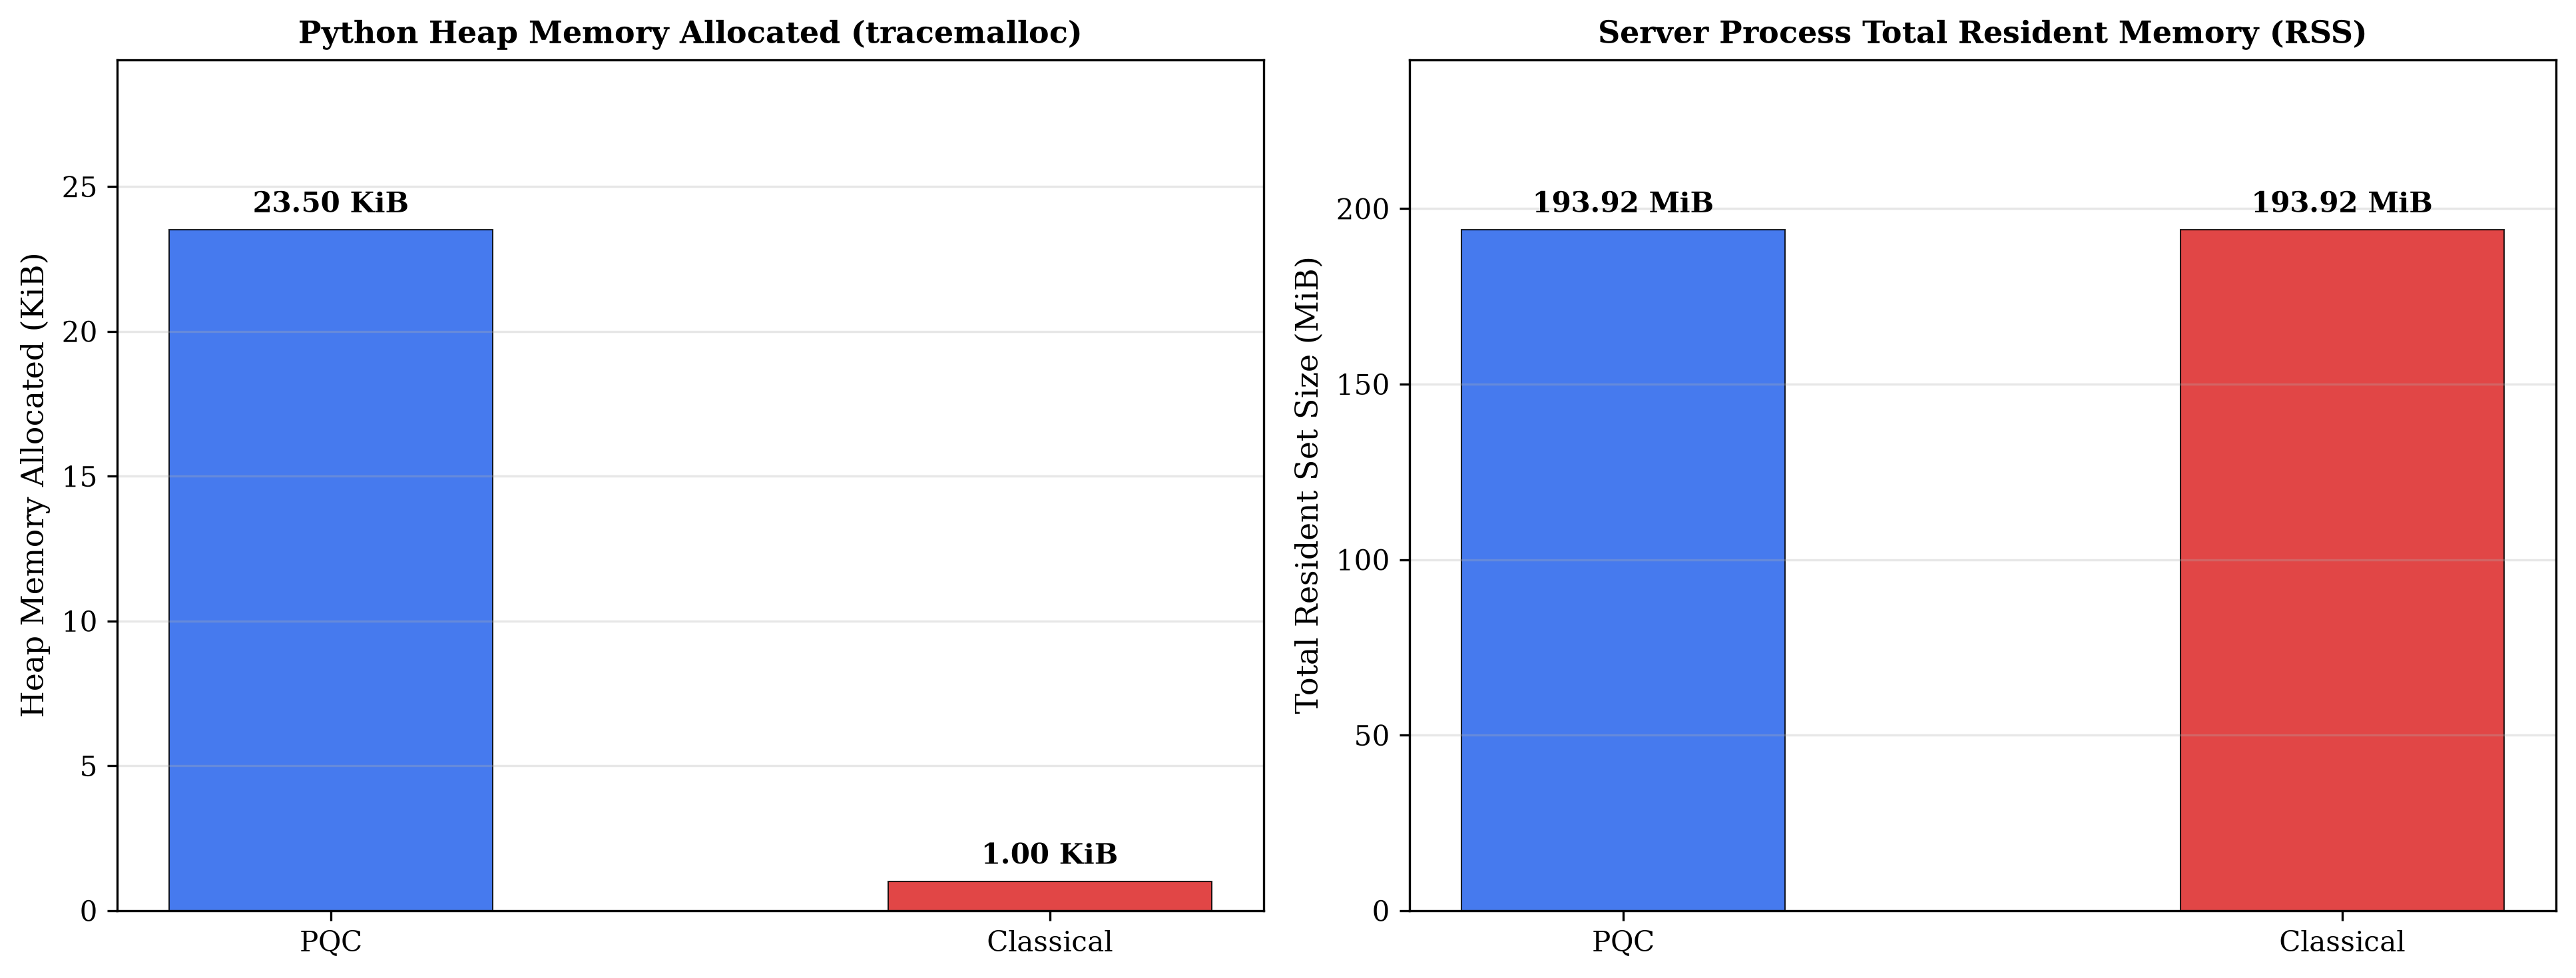
\includegraphics[width=0.85\linewidth]{figures/fig5_memory.png}
\caption{Host Server Memory Profile during Continuous Concurrent Session Handshakes.}
\label{fig:memory_profile}
\end{figure}

\section{Comprehensive Comparative Performance Evaluation}
Table~\ref{tab:perf_comp} synthesizes the empirical performance metrics gathered across all six experimental regimens (E1 through E6).

\begin{table}[htbp]
\centering
\caption{Comprehensive Performance Comparison: Post-Quantum vs Classical Cryptographic Baseline}
\label{tab:perf_comp}
\begin{tabular}{llcc}
\hline
\textbf{Metric} & \textbf{Unit} & \textbf{PQC Path (Mean $\pm$ SD)} & \textbf{Classical Path (Mean $\pm$ SD)} \\
\hline
Keygen Latency & ms & 0.106 $\pm$ 0.015 & 0.090 $\pm$ 0.028 \\
Encapsulation / Agreement & ms & 0.060 $\pm$ 0.007 & 0.085 $\pm$ 0.025 \\
Decapsulation Latency & ms & 0.045 $\pm$ 0.009 & N/A (symmetric scalar mult) \\
Signature Generation (1 KiB) & ms & 0.109 $\pm$ 0.067 & 0.080 $\pm$ 0.039 \\
Signature Verification (1 KiB) & ms & 0.102 $\pm$ 0.101 & 0.250 $\pm$ 0.105 \\
AES-GCM Encryption (1 KiB) & $\mu$s & 3.10 $\pm$ 1.15 & 3.10 $\pm$ 1.15 (Identical) \\
AES-GCM Decryption (1 KiB) & $\mu$s & 2.59 $\pm$ 0.55 & 2.59 $\pm$ 0.55 (Identical) \\
Total Handshake Wire Size & bytes & 10,420 & 304 \\
Server Resident Memory & MiB & 188.86 & 188.86 \\
Quantum Attack Complexity & operations & $> 2^{192}$ (Lattice Hardness) & $O(\log^3 N)$ (Broken by Shor) \\
\hline
\end{tabular}
\end{table}

\section{Summary of Findings}
The empirical results definitively validate the viability of quantum-resistant cryptography within resource-constrained digital microfluidic networks:
\begin{enumerate}
    \item \textbf{Computational Feasibility}: ML-KEM-768 encapsulation is faster than classical X25519, and ML-DSA-65 verification is $2.4\times$ faster than Ed25519.
    \item \textbf{Cyber-Physical Security Assurance}: 100\% of bit-flip assay falsification attacks (Ali et al.) are caught and thwarted before physical actuation; replay attacks are rejected via strictly monotonic nonces.
    \item \textbf{Ephemeral Zero-Retention Footprint}: Conformance to NIST SP 800-57 ensures that zero plaintext key material is persisted to long-term storage, preventing post-compromise key recovery.
\end{enumerate}
